\section{From guarded hMSC to pure LTS\label{section:deductive-glts-to-lts}}

This section presents algorithms for explicitly capturing the traces of a guarded hMSC through a pure LTS. Section \ref{subsection:from-ghmsc-to-glts} provides an algorithm for transforming a g-hMSC into a g-LTS. Section \ref{subsection:from-glts-to-lts} then shows how the set of event traces admitted by a g-LTS can be captured through a LTS.

\subsection{From guarded hMSC to guarded LTS\label{subsection:from-ghmsc-to-glts}}

A guarded hMSC can be transformed into an equivalent g-LTS. The latter abstracts from the agents and captures the set of global behaviors covered by the g-hMSC. The transformation algorithm extends the technique introduced in Section \ref{subsection:background-hmsc} to synthesize a LTS capturing the traces of hMSC \cite{Uchitel:2004}. 

Our algorithm is illustrated in Fig.~\ref{image:scheduler-ghmsc-glts} for the guarded hMSC in Fig.~\ref{image:scheduler-ghmsc}.

\noindent \textbf{Handling nodes} -- Every hMSC node yields a behaviorally equivalent sub-LTS.
\begin{enumerate}[(a)]
\item A terminal MSC node is transformed into a sub-LTS collecting the linear event sequence from the scenario. For a MSC $M$, the LTS captures the set of traces $\mathcal{L}_{total}(M)$ defined in Section \ref{subsection:background-positive-scenarios}.
\item For a node expanded into a finer-grained hMSC, the procedure is applied recursively to obtain the corresponding sub-LTS.
\item A decision node is rewritten as a sub-LTS reduced to one simple state and no event. The same applies to the \emph{start} and \emph{end} nodes of the hMSC.
\end{enumerate}

In cases (a) and (b), the $Task_{start}$ and $Task_{end}$ special events are added as first and last events of the corresponding sub-LTS, respectively.

\noindent \textbf{Handling edges} -- The edges in the guarded hMSC yield transitions between the \emph{terminal} and \emph{initial} states of the sub-LTS corresponding to their \emph{source} and \emph{target} nodes, respectively.
\begin{itemize}
\item An outgoing edge of a decision node is further labeled by the corresponding guard to yield a guarded transition in the g-LTS.
\item Any other edge is simply converted to a $\tau$ transition.
\end{itemize}

\begin{figure}[H]\centering
\scalebox{0.57}{
  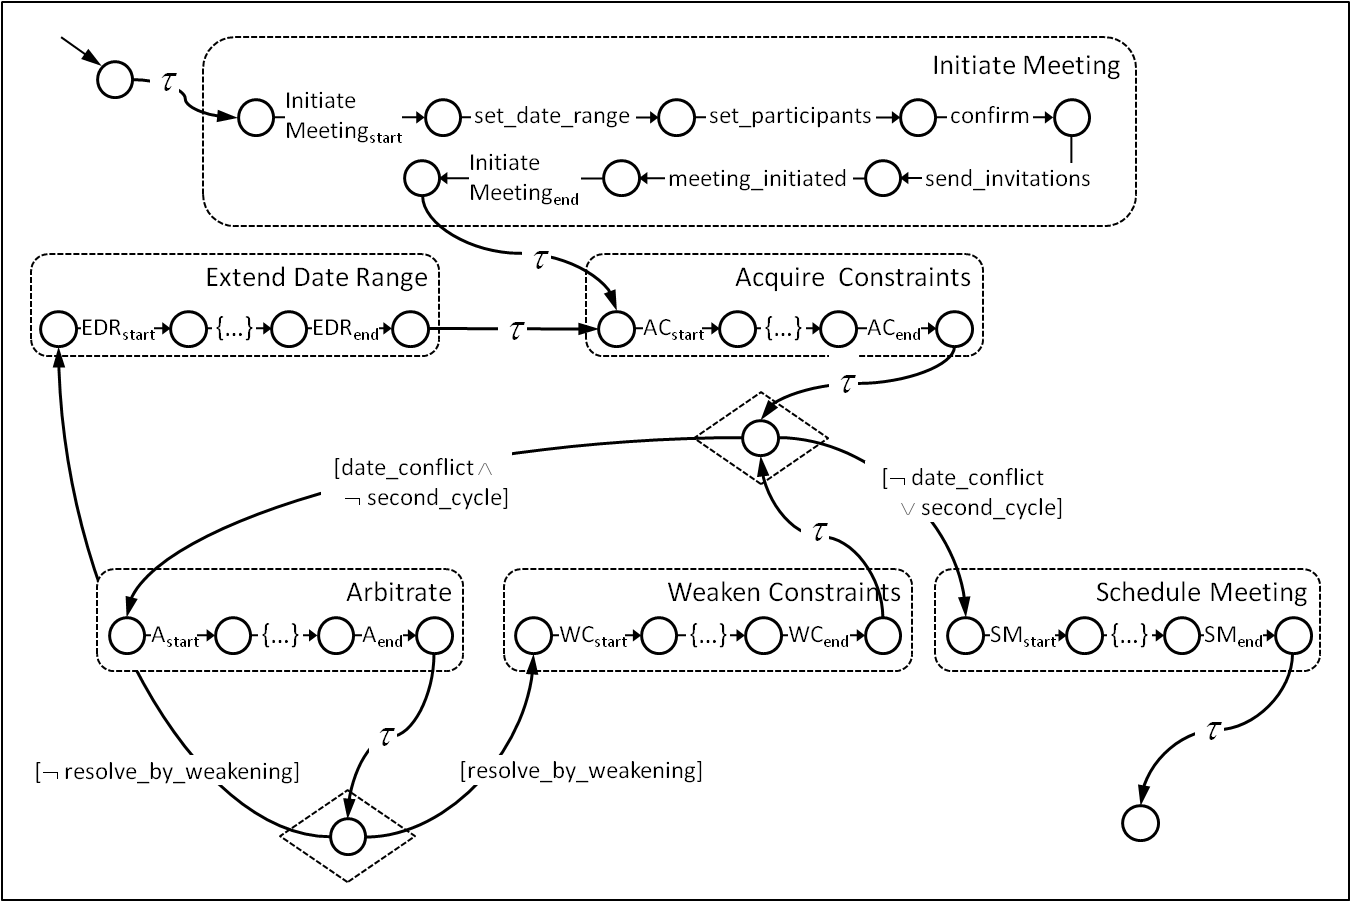
\includegraphics[trim=2mm 2mm 2mm 2mm, clip]{src/3-deductive/images/ghmsc-glts-scheduler}
}
\caption{Transforming a g-hMSC into a g-LTS: the meeting scheduler example from Fig.~\ref{image:scheduler-ghmsc}.\label{image:scheduler-ghmsc-glts}}
\end{figure}

The resulting g-LTS can be further optimized by coalescing states separated by $\tau$ transitions. The g-LTS state space is thereby reduced; this will speed up the synthesis of a trace-equivalent LTS and the model-checking procedure described in Section \ref{section:tool-model-checker}. 

However, such optimization breaks the traceability between g-hMSC tasks and g-LTS states. Such traceability turn to be useful in practice for providing users with feedback on the submitted process model itself (see Section \ref{section:tool-clinical-pathway-analyzer}). 

\subsection{From guarded LTS to pure LTS\label{subsection:from-glts-to-lts}}

The set of traces accepted by a g-LTS may be captured by a trace-equivalent LTS. To build this LTS, a parallel composition of g-LTSs is computed so as to meet the various acceptance conditions in Section \ref{subsection:glts-trace-semantics}. 

\begin{itemize}
\item The first g-LTS in this composition is a super g-LTS meeting the \emph{trace inclusion} and \emph{admissible start} condition.
\item To meet the \emph{guard satisfaction} condition, the set of traces of the super g-LTS is pruned further by composing it with fluent automata. 
\end{itemize}

Let us make each g-LTS in the composition further precise.

\noindent \textbf{Super g-LTS} -- By definition, the input g-LTS already meets the \emph{trace inclusion} condition. In order to meet the \emph{admissible start} condition, it is extended by converting the initial condition $C_0$ into an explicit guard from the initial state. 

If the input g-LTS is $(Q,\Sigma,\Phi,\delta,q_{0},C_{0})$, the super g-LTS is defined by:
\begin{equation*}
Super~LTS = (Q \cup \{ q_{start} \}, \Sigma, \Phi, \delta \cup \{(q_{start},C_0,q_0)\},q_{start},true)
\end{equation*}

\noindent \textbf{Fluent g-LTS} -- The \emph{guard satisfaction} condition is enforced by pruning all traces violating guards in the super g-LTS. For this we compose the super g-LTS with fluent automata. They keep track of current fluent values and constraint guards accordingly.

Every fluent $Fl = \textless Init_{Fl}, Term_{Fl} \textgreater $ yields a g-LTS $(Q,\Sigma,\Phi,\delta,q_{0},C_{0})$ where:
\begin{align*}
Q      &= \{q_u,q_t,q_f\}            \\
\Sigma &= Init_{Fl} \cup Term_{Fl}   \\
\Phi   &= \{ Fl \} \\
\delta &=    \{~(q_f,e,q_t) \mid e \in Init_{Fl}~\}~\cup \{~(q_t,e,q_t) \mid e \in Init_{Fl}~\} \\
       &\cup~\{~(q_t,e,q_f) \mid e \in Term_{Fl}~\} \cup \{~(q_f,e,q_f) \mid e \in Term_{Fl}~\} \\
       &\cup~\{~(q_u, [Fl], q_t),~(q_u, [\neg Fl], q_f)~\} \\
       &\cup~\{~(q_t, [Fl], q_t),~(q_f, [\neg Fl], q_f)~\} \\
q_0    &= q_u \\
C_0    &= true
\end{align*}

In this definition, $q_u$, $q_t$ and $q_f$ denote g-LTS states where the fluent is \emph{unsassigned}, \emph{true} and \emph{false}, respectively (see Fig.~\ref{image:fluent-glts}). Moreover,

\begin{itemize}
\item The unassigned state $q_u$ is the initial g-LTS state. From there, the true and false states may be reached through guarded transitions that force the fluent to an initial value consistent with the reached state;
\item The g-LTS may transit from its false state $q_f$ to its true state $q_t$ with the occurence of events belonging to $Init_{Fl}$ and vice-versa with events belonging to $Term_{Fl}$. In the figure, a transition labeled with a set between brackets is a shortcut denoting one transition for each element of the set;
\item In each state $q_f$ and $q_t$, a self-looping guard constrains the fluent value to the one denoted by the corresponding state. The conjunction of such guards with the ones of the super g-LTS will force the resulting composition to meet the \emph{guard satisfaction} condition;
\item The two last self-looping transitions labeled with $Init_{Fl}$ and $Term_{Fl}$ are added to avoid over-constraining the composition;
\end{itemize}

\begin{figure}[H]\centering
\scalebox{0.75}{
  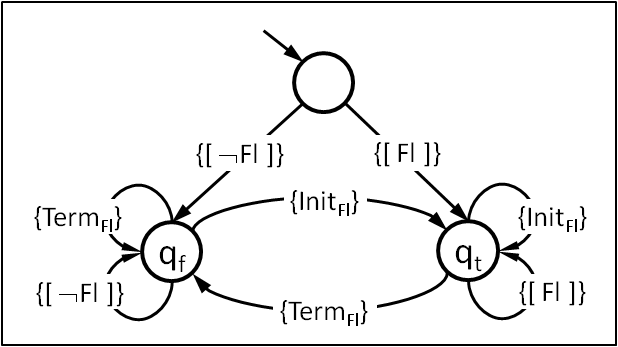
\includegraphics[trim=2mm 2mm 2mm 2mm, clip]{src/3-deductive/images/fluent-glts}
}
\caption{A generic fluent g-LTS\label{image:fluent-glts}}
\end{figure}

For example, consider the following fluent for the meeting scheduler exemplar:
\begin{center}
fluent $second\_cycle = \textless \{ ExtendDateRange_{end}, \newline WeakenConstraints_{end} \},
 \{ InitiateMeeting_{end} \} \textgreater $\\
\end{center}

The corresponding fluent automaton is shown in Fig.~\ref{image:second-cycle-fluent-glts}:

\begin{figure}[H]\centering
\scalebox{0.75}{
  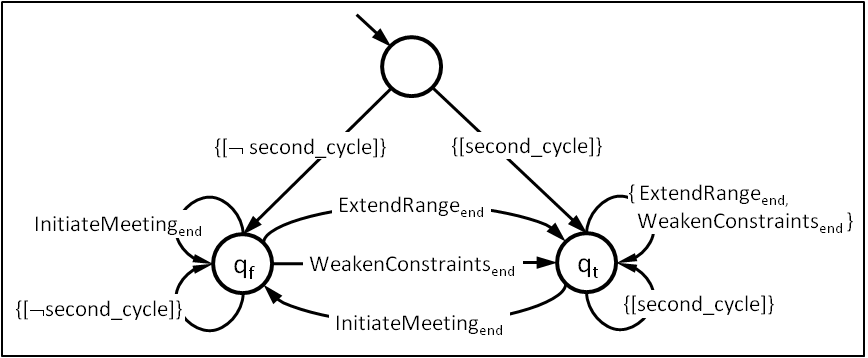
\includegraphics[trim=2mm 2mm 2mm 2mm, clip]{src/3-deductive/images/second-cycle-fluent-glts}
}
\caption{Fluent g-LTS for $second\_cycle$\label{image:second-cycle-fluent-glts}}
\end{figure}

\noindent \textbf{Synthesized LTS} -- Putting pieces together, the trace-equivalent LTS of a g-LTS is obtained through the following computation:
\begin{align*}
\left((Super~LTS \parallel G_{Fl_1} \parallel \ldots \parallel G_{Fl_n}) \setminus \mathcal{P}(2^\Phi)\right)^\Delta
\end{align*}
\noindent where $G_{Fl_i}$ denotes the fluent automaton of the i-th fluent and $\Delta$ is the LTS operator that transforms any LTS into its canonical form through determinization and minimization (see Section~\ref{section:background-state-machines}).

\noindent To sum up, 
\begin{itemize}
\item a g-LTS is first obtained through the composition of the Super LTS with fluent automata; 
\item all guards are then hidden, resulting in a pure LTS;
\item the latter can be further determinized and minimized into its canonical form;
\end{itemize}

Figure \ref{image:scheduler-lts} shows the resulting LTS obtained on the meeting scheduling example from Fig.~\ref{image:scheduler-ghmsc}. The task refinements are not entirely unfolded there; only events used in fluent definitions were kept. The \artifact{no\_remaining\_solution} event, for example, denotes an initiating event of the \artifact{date\_conflict} fluent; it belongs to the refinement of the \artifact{AcquireConstraints} tasks. The events \artifact{click\_extend} and \artifact{click\_weaken} suggest buttons allowing the meeting initiator to select resolution heuristics when a conflict occurs. They appear in the definition of the fluent \artifact{resolve\_by\_weakening}. A transition labeled with `$\ldots$' denotes a sequence of events not shown for readability.

Unlike the original g-hMSC and its g-LTS reformulation, this LTS does not contain any loop. This happens because the $second\_cycle$ fluent prevents looping in indefinite meeting arbitrations. In other words, in our example the technique unfolds the process models as three possible scenarios. In the right most one, no date conflict arises and the meeting is scheduled immediately after having acquired the constraints. In the middle one, a conflict occurs and is resolved by weakening the participant constraints. In the left most one, the resolution consists in extending the date range and collecting constraints one again. In the last two cases, even if the absence of an optimal solution triggers a new date conflict, the meeting is scheduled. 

\begin{figure}\centering
\scalebox{0.15}{
  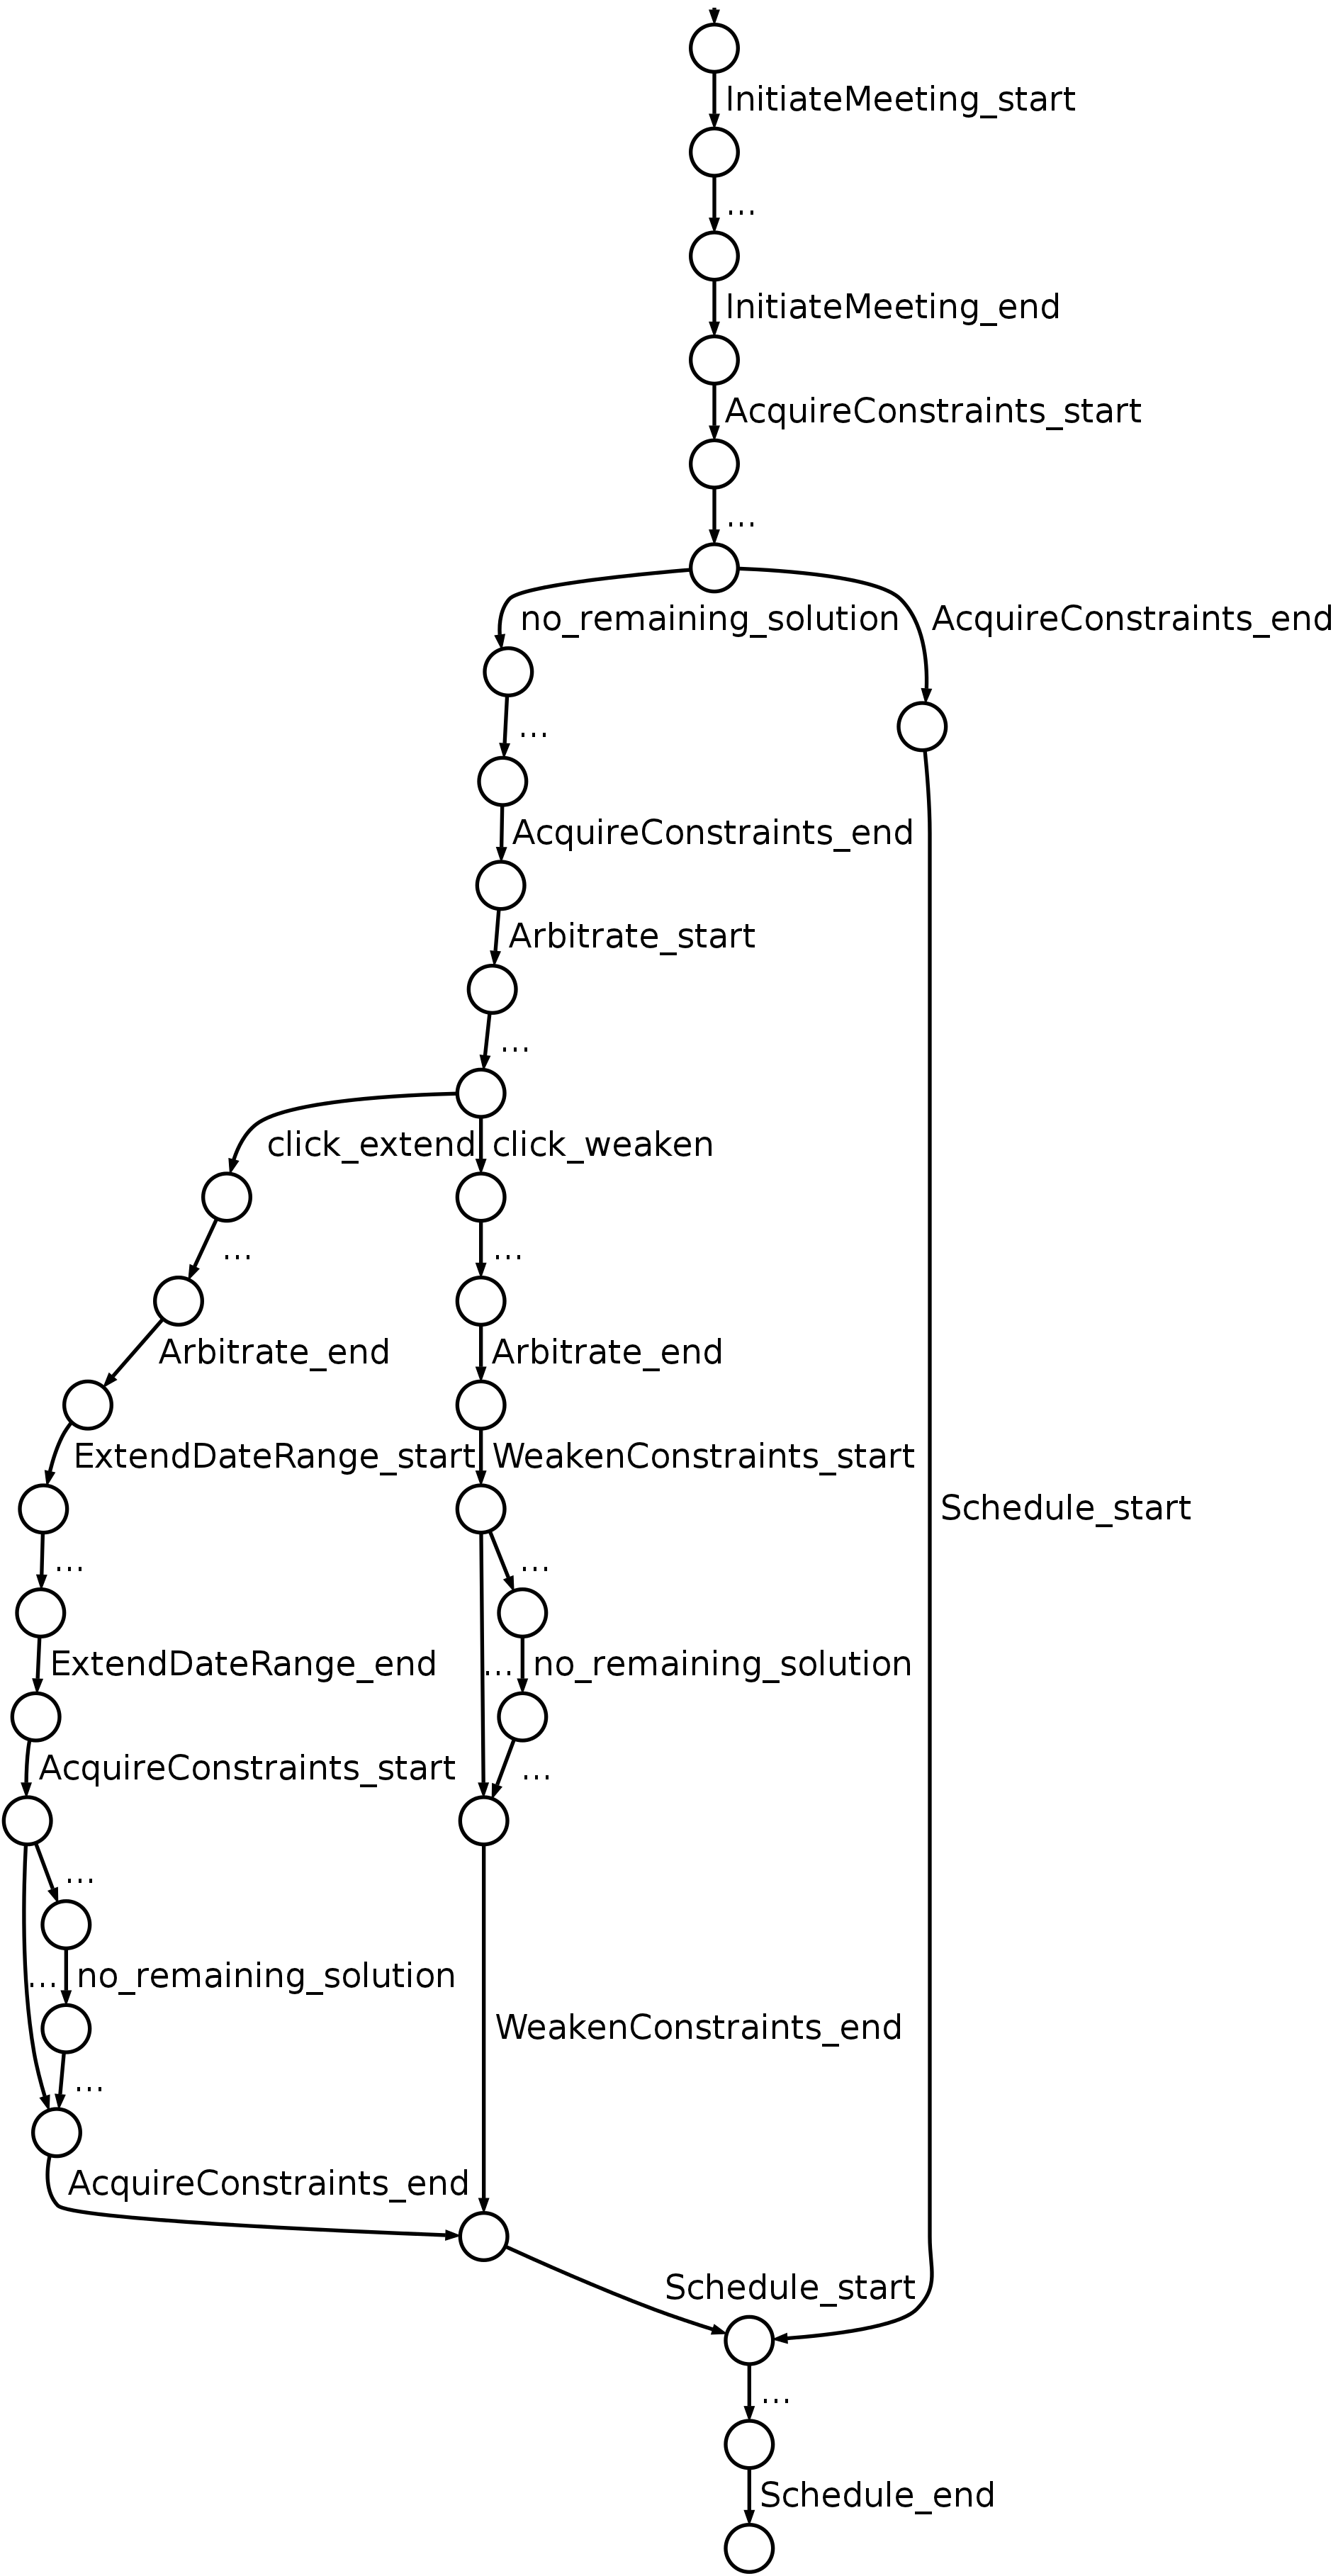
\includegraphics[trim=2mm 2mm 2mm 2mm, clip]{src/3-deductive/images/scheduler-lts}
}
\caption{Trace-equivalent LTS for the meeting scheduling example from Fig.~\ref{image:scheduler-ghmsc}.\label{image:scheduler-lts}}
\end{figure}

Note that our composition technique always considers $2^{\mid\Phi\mid}$ initial fluent assignments, pruning those that do not satisfy $C_0$. In practice, certain fluents have a specific initial value; in this case, the corresponding fluent automaton can be optimized by removing a transition from its initial state. This allows us to avoid computing some of the unsatisfiable conjunctions on the global initial state. The approach might even be improved so as to consider only fluent initializations satisfying $C_0$. If such optimization speeds up the computation in practice, the exponential blow of the resulting trace LTS remains unavoidable. It naturally results from the ability of models with guards to cover numerous behaviors in an implicit, compact way. 
